\documentclass[master=elt,masteroption=eg,dutch,oneside]{kulemt}
\setup{title={Systeemontwerp met HDL},
  subtitle={Audio spectrum analyzer met HDMI uitvoer},
  author={Gert-Jan Andries\and Xavier Dejager\and Nick Steen},
  promotor={Sammy Verslype},
  assessor={Sammy Verslype},
  assistant={Sammy Verslype}}

\usepackage{graphicx}
\usepackage{titlesec}
\usepackage{listings}
\usepackage{color}
\usepackage{float}
\usepackage{amsmath}
\usepackage{booktabs}
\usepackage{upquote}
\usepackage{gensymb}
\usepackage{cite}
\usepackage{setspace}
\usepackage{subcaption}

\setlength{\parskip}{1em}
\setlength\parindent{0pt}

\titleformat{\chapter}[display]
    {\normalfont\huge\bfseries}{\chaptertitlename\ \thechapter}{20pt}{\Huge}
\titlespacing*{\chapter}{0pt}{-25pt}{10pt}

\begin{document}
	\tableofcontents*
	\chapter{Afkortingen en symbolen}
\section*{Afkortingen}
\begin{flushleft}
  \renewcommand{\arraystretch}{1.1}
  \begin{tabularx}{\textwidth}{@{}p{12mm}X@{}}
        ADC     & Analoog - Digitaalconverter                           \\													
        ASCII   & American Standard Code for Information Interchange    \\													
        AXI		& Advanced Extensible Interface							\\				
        CS		& Chip Select											\\
        DFT     & Discrete Fourier Transformatie                        \\													
        DSP     & Digital Signal Processing                             \\													
        FFT     & Fast Fourier Transformatie                            \\													
        FPGA    & Field-Programmable Gate Array                         \\													
        HDL     & Hardware Description Language                         \\													
        HDMI    & High Definition Multimedia Interface                  \\													
        I\textsuperscript{2}C     & Inter Integrated Circuit bus        \\													
        I\textsuperscript{2}S     & Inter Integrated Circuit Sound      \\													
        IP      & Intellectual Property                                 \\													
        LED 	& Light Emitting Diode									\\			
        LSB     & Least Significant Bit                                 \\													
        MSB     & Most Significant Bit                                  \\													
        OLED    & Organic Light Emitting Diode                          \\													
        PLL     & Phase-Locked Loop                                     \\													
        RAM     & Random Acces Memory                                   \\													
        RGB     & Red Green Blue / Rood Groen Blauw                     \\													
        ROM     & Read Only Memory                                      \\													
        SCL     & Serial Clock                                          \\													
        SDA     & Serial Data                                           \\													
        SPI     & Serial Peripheral Interface                           \\													
        VGA     & Video Graphics Array                                  \\													
        VHDL    & VHSIC Hardware Description Language                   \\													
        VHSIC   & Very High Speed Integrated Circuit                    \\													
        YCbCr   & Luminance Chrominance                                 \\									
  \end{tabularx}
\end{flushleft}

	\mainmatter
	\chapter{Inleiding}

\par Tijdens de lessenreeks systeemontwerp met HDL werd kennis gemaakt met de Xilinx Vivado ontwikkelomgeving. Onder meer volgende topics kwamen aan bod:
	
		\begin{description}
			\item[Simulatie en constraints:] In dit hoofdstuk werden constraints en simulaties in de Vivado omgeving behandeld. Hiernaast kwam ook het ZedBoard ontwikkelbord aan bod.
			\item[IP en clocking resources:] In dit hoofdstuk werd dieper ingegaan op IP's en hoe deze kunnen worden ge\"integreerd. Verder werd ook gekeken naar klokpaden binnen een ontwerp en het gebruik van de clocking wizard.
			\item[Hardware debugging:] In deze les werd uitgelegd hoe men door middel van een ILA uit de IP catalog een signaal kan monitoren dat zich binnen de FPGA bevindt. 
		\end{description}

\par Na deze theorielessen werd in groep een groter project uitgwerkt op een FPGA-ontwikkelbord (ZedBoard). Dit project bestond eruit om een audio spectrum analyzer te maken. Deze analyzer neemt als invoer een stereo audiosignaal dat wordt binnengelezen via een audiocodec. Vervolgens dient er een spectra van deze signalen berekend te worden op de FPGA (zowel voor de linker als het rechter audiokanaal). Dit spectrum zal dan op een beeldscherm worden weergegeven door middel van een HDMI interface. 

\par Het project kan worden aangevuld met volgende extra features:

		\begin{itemize}
			\item Piek aanduiding (bv. ander kleur of horizontale lijn)
			\item Werken met verschillende kleuren (i.f.v. frequentie of amplitude)
			\item Keuze aan gebruiker over grafiektype (bars, dots, lijn\ldots)
			\item \ldots
		\end{itemize}

\par In dit verslag zal de werking en opbouw van het project overlopen worden. Elke component zal kort worden besproken en ook de moeilijkheden tijdens het ontwerpproces komen aan bod.
	\chapter{Spectrum Analyzer}

\section{Audio}

	\par Audio is een continu variabel en analoog signaal, dat dus niet direct digitaal te verwerken valt.
	Het is vaak niet-periodiek en kan dus niet per periode geanalyseerd worden.
	Om het digitaal te kunnen verwerken, wat uiteindelijk gebeurt bij de interne werking van de FPGA, dient het gesampled te worden, om daarna via een ADC aan de invoer van de digitale schakeling gelegd te worden.

\section{Analyse}

	\par De analyse gebeurt digitaal en via de Fourier transformatie. De Fourier transformatie baseert zich op het feit dat een signaal kan opgedeeld worden in de som van sinussen en cosinussen. Elke sinus of cosinus heeft een eigen frequentie en amplitude, waardoor er dus kan geanalyseerd worden welke frequenties er sterker aangwezig zijn in het ingangssignaal. Gezien het karakter van de audio dient hier met een DFT gewerkt te worden, een transformatie die een eindige periode nodig heeft om een analyse op uit te voeren. Door over een vaste periode te samplen, wordt een window gegenereerd die zo als input kan dienen voor deze transformatie.
	
	\par Gezien de digitale aard van de schakeling en de snelheid die nodig is om de verwerking uit te voeren, is het beter een aantal opeenvolgende samples te kiezen die een macht van 2 zijn. Dit houdt in dat er 2, 4, 8 \ldots samples genomen dienen te worden. Zo kan dan via een sneller algoritme, de FFT, het resultaat berekend worden.

\section{Hamming Window}

	\par Omdat we een FFT willen toepassen in real time moeten we het signaal in stukken hakken. Hoe groter dit stuk hoe beter de lage frequenties kunnen bepaald worden, maar hoe meer delay er komt op de uitgang van het spectrum. En door de aard van het FFT algoritme zal dit stuk als een periodiek herhalend stuk aanzien worden. Nu weten we dat een plotste verandering in amplitude veel hoge spectrale componenten zal bevatten. En omdat het sampelen op een bepaald tijdstip gebreurd kan dit er voor kan zorgen dat het eerste en het laatste sample niet gelijk uitkomen. En mogelijks zelf veel van elkaar verschillen. Daar zal dus een scherpe overgang zijn. Dit effect zal het spectrum aanzienlijk be\"invloeden. Om dit tegen te gaan maken we gebruik van een hamming window. Dit zorgt er voor dat de uiteinden heel geleidelijk naar nul gebracht worden, daardoor is het ommogelijk om daar die plotse overhang te krijgen. Het hamming window zelf heeft ruwweg de vorm van een cosinus:

		\begin{equation}
		 w(n) = \alpha - \beta \cos \left( \frac{2 \pi n}{N-1} \right)
		\end{equation}

	\par Door de samples te convolueren met de het punten van het hamming window bereiken we dat de uiteinden nagenoeg nul zijn op de uiteindes. Merk wel op dat wij de waardes voor de hamming functie gemapt hebben van 0 tot en met 255. Dit omdat het veel eenvoudiger is om integers te vermenigvuldigen dan floating point getallen te vermenigvuldigen op een FPGA.

\section{Uitgang}

	\par Uit de uitgang van de FFT kan dan gehaald worden hoe sterk bepaalde frequenties aanwezig zijn.	Om dit aan de gebruiker duidelijk te maken, kan dit via een grafische output weergegeven worden.
	\chapter{Spectrum Analyzer}

\section{Audio}

	\par Audio is een continu variabel en analoog signaal, dat dus niet direct digitaal te verwerken valt.
	Het is vaak niet-periodiek en kan dus niet per periode geanalyseerd worden.
	Om het digitaal te kunnen verwerken, wat uiteindelijk gebeurt bij de interne werking van de FPGA, dient het gesampled te worden, om daarna via een ADC aan de invoer van de digitale schakeling gelegd te worden.

\section{Analyse}

	\par De analyse gebeurt digitaal en via de Fourier transformatie. De Fourier transformatie baseert zich op het feit dat een signaal kan opgedeeld worden in de som van sinussen en cosinussen. Elke sinus of cosinus heeft een eigen frequentie en amplitude, waardoor er dus kan geanalyseerd worden welke frequenties er sterker aangwezig zijn in het ingangssignaal. Gezien het karakter van de audio dient hier met een DFT gewerkt te worden, een transformatie die een eindige periode nodig heeft om een analyse op uit te voeren. Door over een vaste periode te samplen, wordt een window gegenereerd die zo als input kan dienen voor deze transformatie.
	
	\par Gezien de digitale aard van de schakeling en de snelheid die nodig is om de verwerking uit te voeren, is het beter een aantal opeenvolgende samples te kiezen die een macht van 2 zijn. Dit houdt in dat er 2, 4, 8 \ldots samples genomen dienen te worden. Zo kan dan via een sneller algoritme, de FFT, het resultaat berekend worden.

\section{Hamming Window}

	\par Omdat we een FFT willen toepassen in real time moeten we het signaal in stukken hakken. Hoe groter dit stuk hoe beter de lage frequenties kunnen bepaald worden, maar hoe meer delay er komt op de uitgang van het spectrum. En door de aard van het FFT algoritme zal dit stuk als een periodiek herhalend stuk aanzien worden. Nu weten we dat een plotste verandering in amplitude veel hoge spectrale componenten zal bevatten. En omdat het sampelen op een bepaald tijdstip gebreurd kan dit er voor kan zorgen dat het eerste en het laatste sample niet gelijk uitkomen. En mogelijks zelf veel van elkaar verschillen. Daar zal dus een scherpe overgang zijn. Dit effect zal het spectrum aanzienlijk be\"invloeden. Om dit tegen te gaan maken we gebruik van een hamming window. Dit zorgt er voor dat de uiteinden heel geleidelijk naar nul gebracht worden, daardoor is het ommogelijk om daar die plotse overhang te krijgen. Het hamming window zelf heeft ruwweg de vorm van een cosinus:

		\begin{equation}
		 w(n) = \alpha - \beta \cos \left( \frac{2 \pi n}{N-1} \right)
		\end{equation}

	\par Door de samples te convolueren met de het punten van het hamming window bereiken we dat de uiteinden nagenoeg nul zijn op de uiteindes. Merk wel op dat wij de waardes voor de hamming functie gemapt hebben van 0 tot en met 255. Dit omdat het veel eenvoudiger is om integers te vermenigvuldigen dan floating point getallen te vermenigvuldigen op een FPGA.

\section{Uitgang}

	\par Uit de uitgang van de FFT kan dan gehaald worden hoe sterk bepaalde frequenties aanwezig zijn.	Om dit aan de gebruiker duidelijk te maken, kan dit via een grafische output weergegeven worden.
	\chapter{Spectrum Analyzer}

\section{Audio}

	\par Audio is een continu variabel en analoog signaal, dat dus niet direct digitaal te verwerken valt.
	Het is vaak niet-periodiek en kan dus niet per periode geanalyseerd worden.
	Om het digitaal te kunnen verwerken, wat uiteindelijk gebeurt bij de interne werking van de FPGA, dient het gesampled te worden, om daarna via een ADC aan de invoer van de digitale schakeling gelegd te worden.

\section{Analyse}

	\par De analyse gebeurt digitaal en via de Fourier transformatie. De Fourier transformatie baseert zich op het feit dat een signaal kan opgedeeld worden in de som van sinussen en cosinussen. Elke sinus of cosinus heeft een eigen frequentie en amplitude, waardoor er dus kan geanalyseerd worden welke frequenties er sterker aangwezig zijn in het ingangssignaal. Gezien het karakter van de audio dient hier met een DFT gewerkt te worden, een transformatie die een eindige periode nodig heeft om een analyse op uit te voeren. Door over een vaste periode te samplen, wordt een window gegenereerd die zo als input kan dienen voor deze transformatie.
	
	\par Gezien de digitale aard van de schakeling en de snelheid die nodig is om de verwerking uit te voeren, is het beter een aantal opeenvolgende samples te kiezen die een macht van 2 zijn. Dit houdt in dat er 2, 4, 8 \ldots samples genomen dienen te worden. Zo kan dan via een sneller algoritme, de FFT, het resultaat berekend worden.

\section{Hamming Window}

	\par Omdat we een FFT willen toepassen in real time moeten we het signaal in stukken hakken. Hoe groter dit stuk hoe beter de lage frequenties kunnen bepaald worden, maar hoe meer delay er komt op de uitgang van het spectrum. En door de aard van het FFT algoritme zal dit stuk als een periodiek herhalend stuk aanzien worden. Nu weten we dat een plotste verandering in amplitude veel hoge spectrale componenten zal bevatten. En omdat het sampelen op een bepaald tijdstip gebreurd kan dit er voor kan zorgen dat het eerste en het laatste sample niet gelijk uitkomen. En mogelijks zelf veel van elkaar verschillen. Daar zal dus een scherpe overgang zijn. Dit effect zal het spectrum aanzienlijk be\"invloeden. Om dit tegen te gaan maken we gebruik van een hamming window. Dit zorgt er voor dat de uiteinden heel geleidelijk naar nul gebracht worden, daardoor is het ommogelijk om daar die plotse overhang te krijgen. Het hamming window zelf heeft ruwweg de vorm van een cosinus:

		\begin{equation}
		 w(n) = \alpha - \beta \cos \left( \frac{2 \pi n}{N-1} \right)
		\end{equation}

	\par Door de samples te convolueren met de het punten van het hamming window bereiken we dat de uiteinden nagenoeg nul zijn op de uiteindes. Merk wel op dat wij de waardes voor de hamming functie gemapt hebben van 0 tot en met 255. Dit omdat het veel eenvoudiger is om integers te vermenigvuldigen dan floating point getallen te vermenigvuldigen op een FPGA.

\section{Uitgang}

	\par Uit de uitgang van de FFT kan dan gehaald worden hoe sterk bepaalde frequenties aanwezig zijn.	Om dit aan de gebruiker duidelijk te maken, kan dit via een grafische output weergegeven worden.
	\chapter{Spectrum Analyzer}

\section{Audio}

	\par Audio is een continu variabel en analoog signaal, dat dus niet direct digitaal te verwerken valt.
	Het is vaak niet-periodiek en kan dus niet per periode geanalyseerd worden.
	Om het digitaal te kunnen verwerken, wat uiteindelijk gebeurt bij de interne werking van de FPGA, dient het gesampled te worden, om daarna via een ADC aan de invoer van de digitale schakeling gelegd te worden.

\section{Analyse}

	\par De analyse gebeurt digitaal en via de Fourier transformatie. De Fourier transformatie baseert zich op het feit dat een signaal kan opgedeeld worden in de som van sinussen en cosinussen. Elke sinus of cosinus heeft een eigen frequentie en amplitude, waardoor er dus kan geanalyseerd worden welke frequenties er sterker aangwezig zijn in het ingangssignaal. Gezien het karakter van de audio dient hier met een DFT gewerkt te worden, een transformatie die een eindige periode nodig heeft om een analyse op uit te voeren. Door over een vaste periode te samplen, wordt een window gegenereerd die zo als input kan dienen voor deze transformatie.
	
	\par Gezien de digitale aard van de schakeling en de snelheid die nodig is om de verwerking uit te voeren, is het beter een aantal opeenvolgende samples te kiezen die een macht van 2 zijn. Dit houdt in dat er 2, 4, 8 \ldots samples genomen dienen te worden. Zo kan dan via een sneller algoritme, de FFT, het resultaat berekend worden.

\section{Hamming Window}

	\par Omdat we een FFT willen toepassen in real time moeten we het signaal in stukken hakken. Hoe groter dit stuk hoe beter de lage frequenties kunnen bepaald worden, maar hoe meer delay er komt op de uitgang van het spectrum. En door de aard van het FFT algoritme zal dit stuk als een periodiek herhalend stuk aanzien worden. Nu weten we dat een plotste verandering in amplitude veel hoge spectrale componenten zal bevatten. En omdat het sampelen op een bepaald tijdstip gebreurd kan dit er voor kan zorgen dat het eerste en het laatste sample niet gelijk uitkomen. En mogelijks zelf veel van elkaar verschillen. Daar zal dus een scherpe overgang zijn. Dit effect zal het spectrum aanzienlijk be\"invloeden. Om dit tegen te gaan maken we gebruik van een hamming window. Dit zorgt er voor dat de uiteinden heel geleidelijk naar nul gebracht worden, daardoor is het ommogelijk om daar die plotse overhang te krijgen. Het hamming window zelf heeft ruwweg de vorm van een cosinus:

		\begin{equation}
		 w(n) = \alpha - \beta \cos \left( \frac{2 \pi n}{N-1} \right)
		\end{equation}

	\par Door de samples te convolueren met de het punten van het hamming window bereiken we dat de uiteinden nagenoeg nul zijn op de uiteindes. Merk wel op dat wij de waardes voor de hamming functie gemapt hebben van 0 tot en met 255. Dit omdat het veel eenvoudiger is om integers te vermenigvuldigen dan floating point getallen te vermenigvuldigen op een FPGA.

\section{Uitgang}

	\par Uit de uitgang van de FFT kan dan gehaald worden hoe sterk bepaalde frequenties aanwezig zijn.	Om dit aan de gebruiker duidelijk te maken, kan dit via een grafische output weergegeven worden.
	\chapter{Besluit}
	\section{Sampelen van audio}
		\par Bij het bouwen van een audio spectrum analyzer wordt al snel duidelijk dat je ergens een audiosignaal zal moeten samplen en op \'e\'en of ander manier zal moeten inlezen. Om audio binnen te lezen werd een codec ter beschikking gesteld. Deze codec werd vervolgens uitgebreid zodat het ook mogelijk werd om audio terug uit te sturen. De moeilijkheden die hierbij ondervonden werden waren vornamelijk te wijten aan de beperkte data die beschikbaar was in de datasheet. Door middel van het programma Sigma Studio was het vervolgens wel relatief eenvoudig om de juiste registerinstellingen te maken.

	\section{Dataverwerking en FFT}
		\par Om een spectrum te krijgen van een gesampled signaal moet je er mee rekenen. En een bijkomende moeilijkheid was de vereiste dat de schakeling real time moet werken. Dus met wat we toen al wisten moesten we een algoritme voor een fourier transformatie implementeren en het moest ook snel genoeg zijn om real time te zijn. Daar konden we ons beroepen op de IP library van Xilinx. Deze bevat een FFT blok, die welliswaar via AXI-bus aan te spreken is. De moeilijkheden bij de implementatie van de FFT blok beperkten zicht voornamelijk tot het juist krijgen van de timings van de verschillende signalen.

	\section{Spectrum visualiseren}
		\par Om het scherm aan te sturen waren er ook wat moeilijkheden. Op het eerste maakte het niet uit of we dan wel niet HDMI zouden gebruiken. VGA zou makkelijker zijn volgens zekere bronnen. Uiteindelijk zijn we met HDMI verder gegaan. Toch wel met dank aan een stuk voorbeeldcode gevonden op een forum zijn we dan toch aan de slag kunnen gaan. Eens we ons eerste blok op het scherm konden tekenen ging het steeds vlotter. Hoe meer we de code begrepen hoe meer we de code gingen verbouwen. Tot dat het dan weer totaal misliep, om dan een stap terug te zetten en het nog eens te proberen. 

	\section{OLED display}
		\par Het ontwerpen van de HDMI uitvoer en het OLED scherm gebeurde in twee verschillende projecten. Bij het samenvoegenvan deze projecten werd opgemerkt dat de datapin van het OLED signaal ook verbonden was met een datapin van de HDMI codec. Aanvankelijk werd er geopteerd om ofwel de data te multiplexen. De seri\"ele kloklijnen zouden dan om de beurt op 0 geschakeld worden. Uitijndelijk bleek dat de pin die verbonden was met de HDMI codec steeds op 0 stond en niet actief gebruikt werd. Deze pin maakt deel ui van een 16 bit brede data-interface waarvan enkel de 8 laatste bits in gebruik waren. De gemeenschappelijk pin bevond zich in de eerste 8, ongebruikt pinnen. Een test wees verovolgens uit dat deze data mocht overschreven worden zonder dat dit een invloed gaf op de HDMI uitvoer. Wel moest de OLED data geplaatst worden op een ODDR block omdat de HDMI pinnen via dit principe werkten. 

	\section{VHDL toolbox}
		\par Aan de hand van een kleine toolbox die ontwikkeld werd door middel van C\textsuperscript{\texttt{\#}} gemaakt werd was het op een snelle manier mogelijk om data te genereren voor de verschillende geheugens. Zo wordt onder meer tekstdata voor het OLED scherm automatisch gegenereerd en passend gemaakt voor het geheugen. Ook voor het gradi\"entgeheugen kon data gegenereerd worden op basis van een afbeelding.

	\section{Algemeen}
		\par Algemeen kunnen we stellen dat het een leerzaam project was. Gaande van niks kunnen op een fysisch FPGA development board tot een werkende audio spectrum analyzer was een vrij steile leercurve. Maar eens het eerste gelukt is volgt de rest vrij vlot. Het was vooral een kwestie van die knop om te zetten in ons hoofd. Een tweede moeilijkheid was de omgeving. Op het eerst een overdonderende indruk, een chaos aan features die naderhand uiterst praktisch bleken te zijn. We kunnen zeker stellen dat in de eerste plaats het doel, de opdracht voldaan is. Zelfs met hier een daar een uitbreiding. En in een tweede plaats heeft het zeker en vast een deur wagenwijd opengezet om zelf te gaan experimenteren met de kracht van hardware.
	\appendixpage*
	\appendix
	\addtocontents{toc}{\protect\newpage}
\chapter{Overzicht spectrum analyzer}
\label{sec:appMapping}
	\begin{figure}[H]
		\centering
		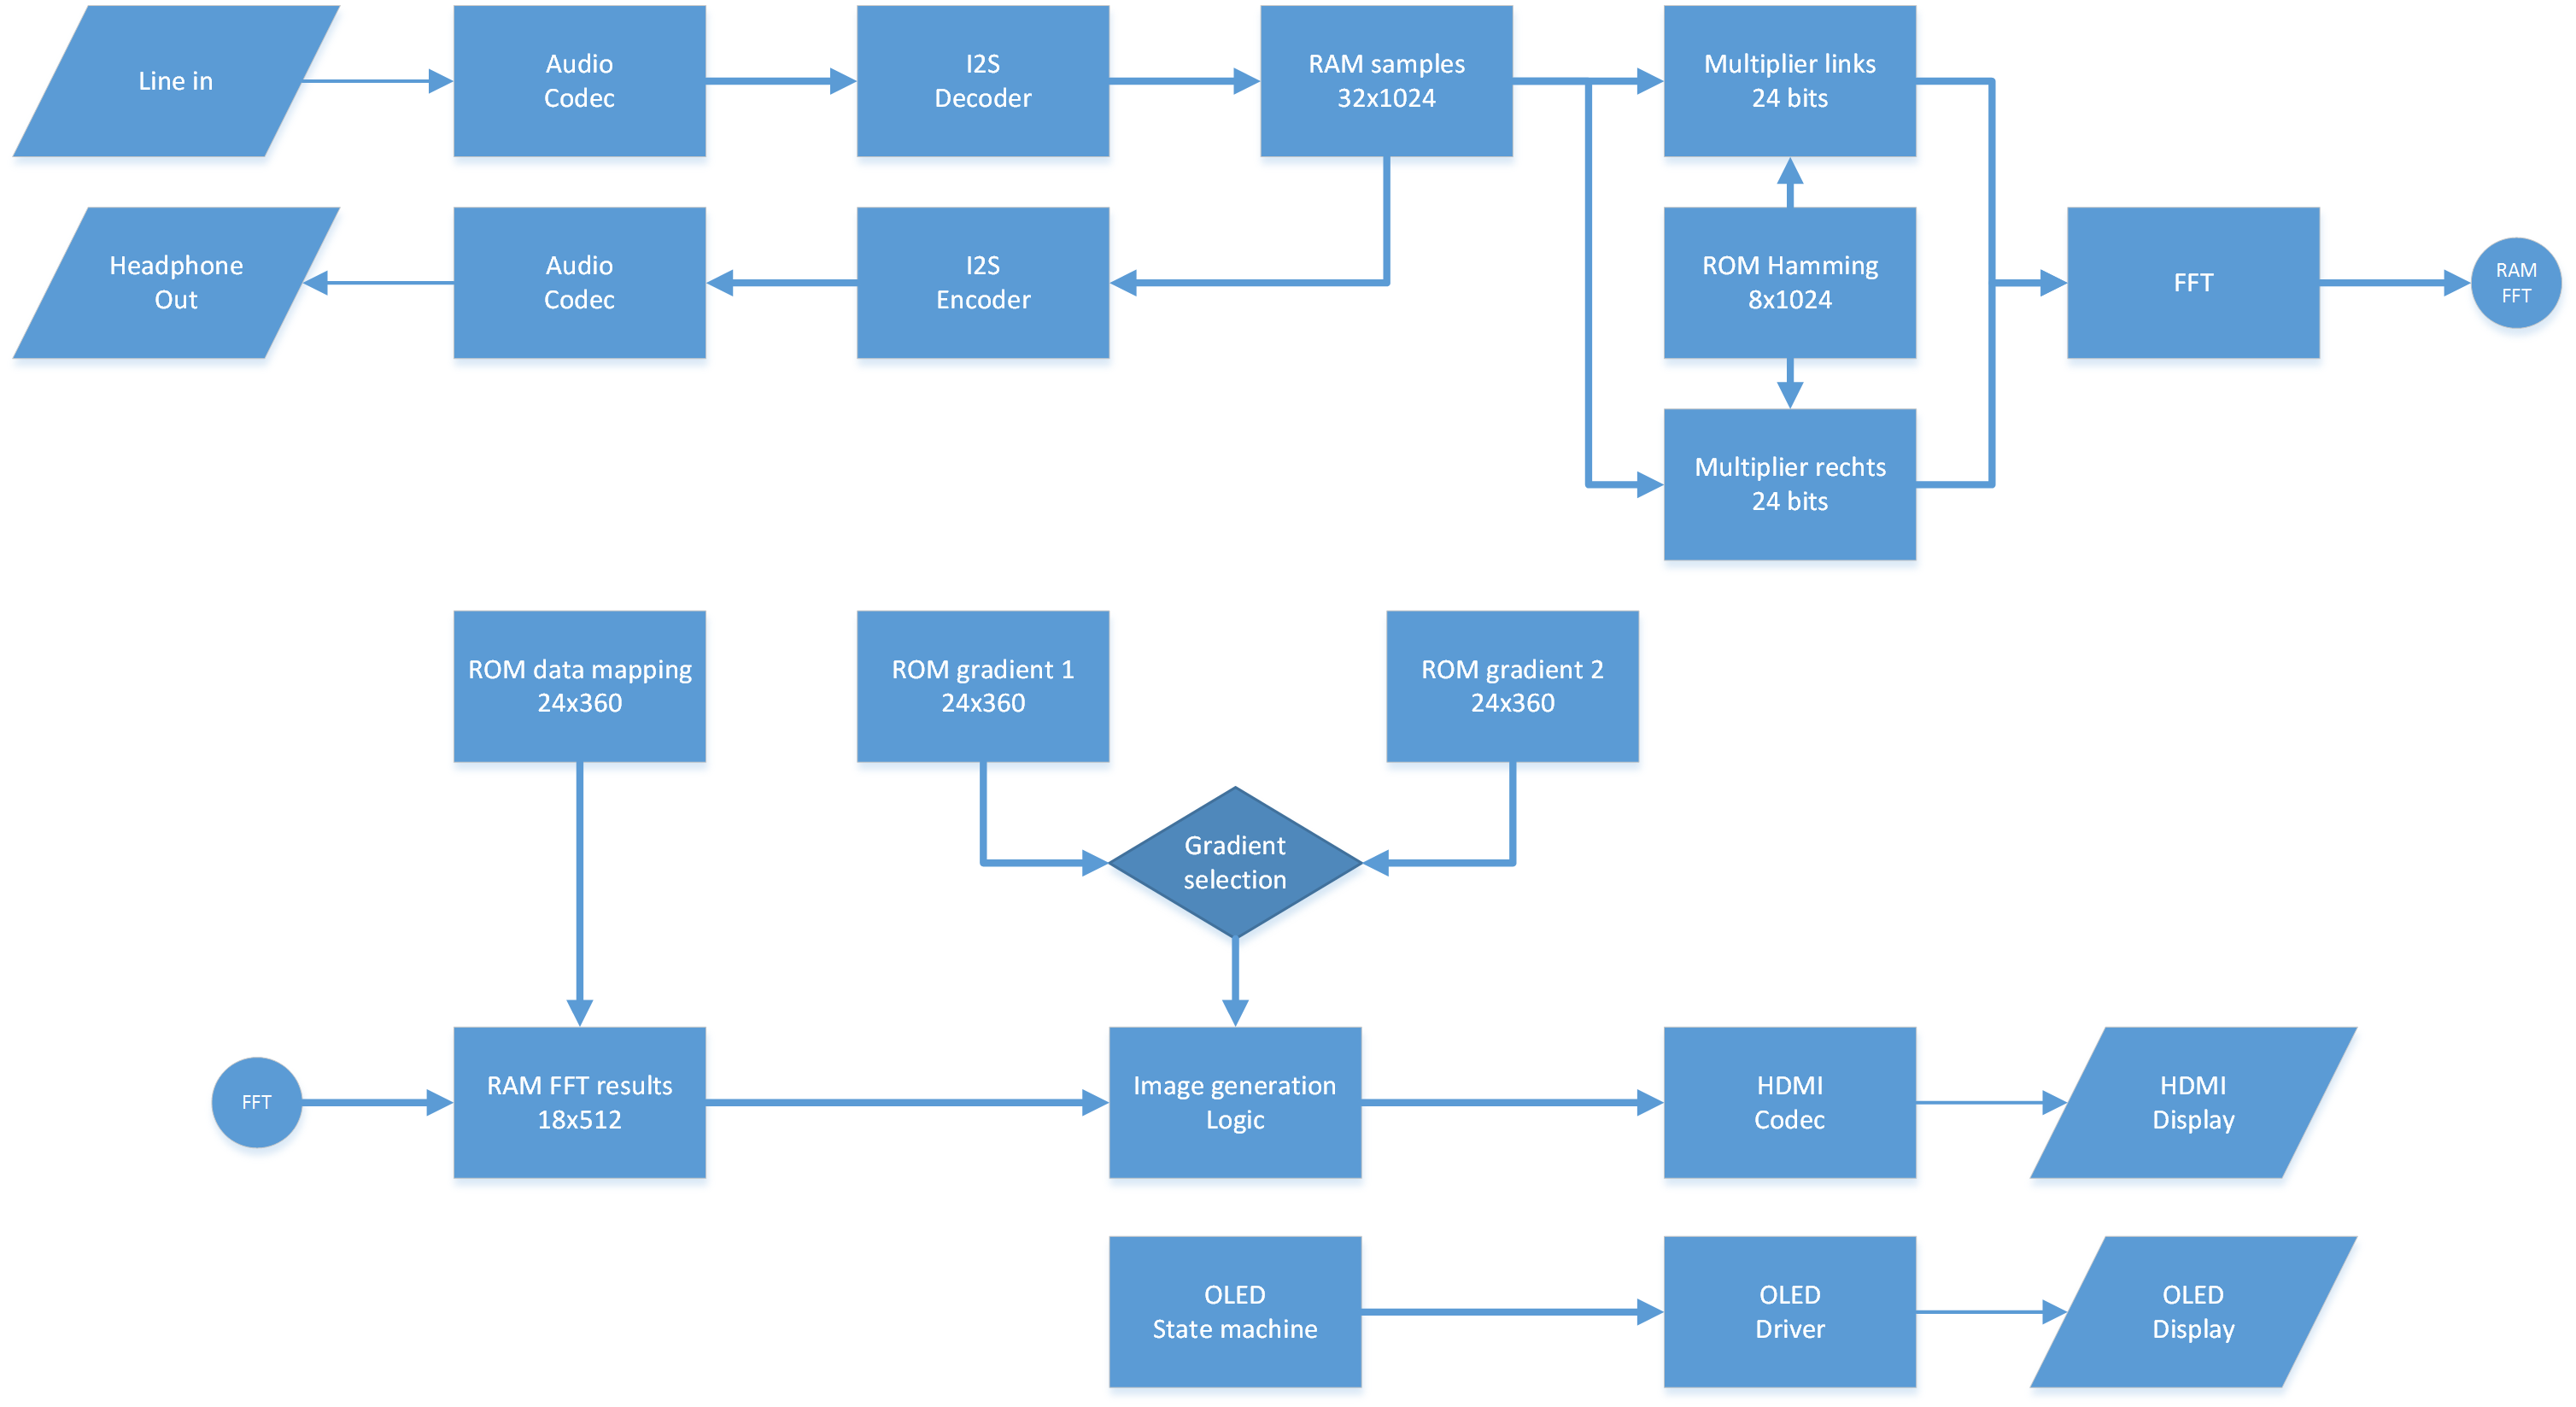
\includegraphics[width=0.75\textheight, angle=270]{Appendix/FlowCharts/Global}
		\caption{Globaal overzicht van de spectrum analyzer}
		\label{fig:FlowChartMapping}
	\end{figure}

\chapter{Componenten}
\section{Top}
\label{sec:appTop}
	\begin{figure}[H]
		\centering
		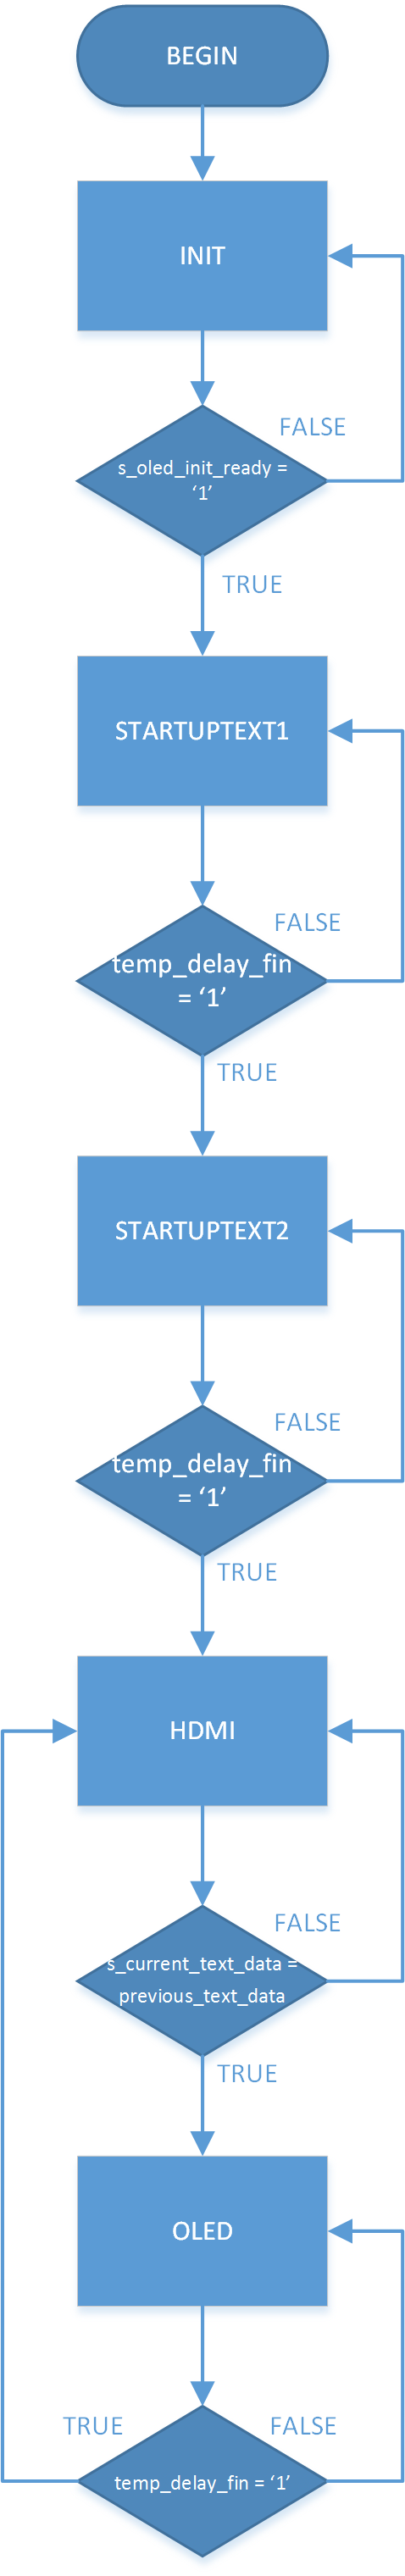
\includegraphics[height=0.66\textheight]{Appendix/FlowCharts/Top}
		\caption{Flowchart van top}
		\label{fig:FlowChartTop}
	\end{figure}

\newpage
\section{Audio interface}
\label{sec:appAudioIf}
	\begin{figure}[H]
		\centering
		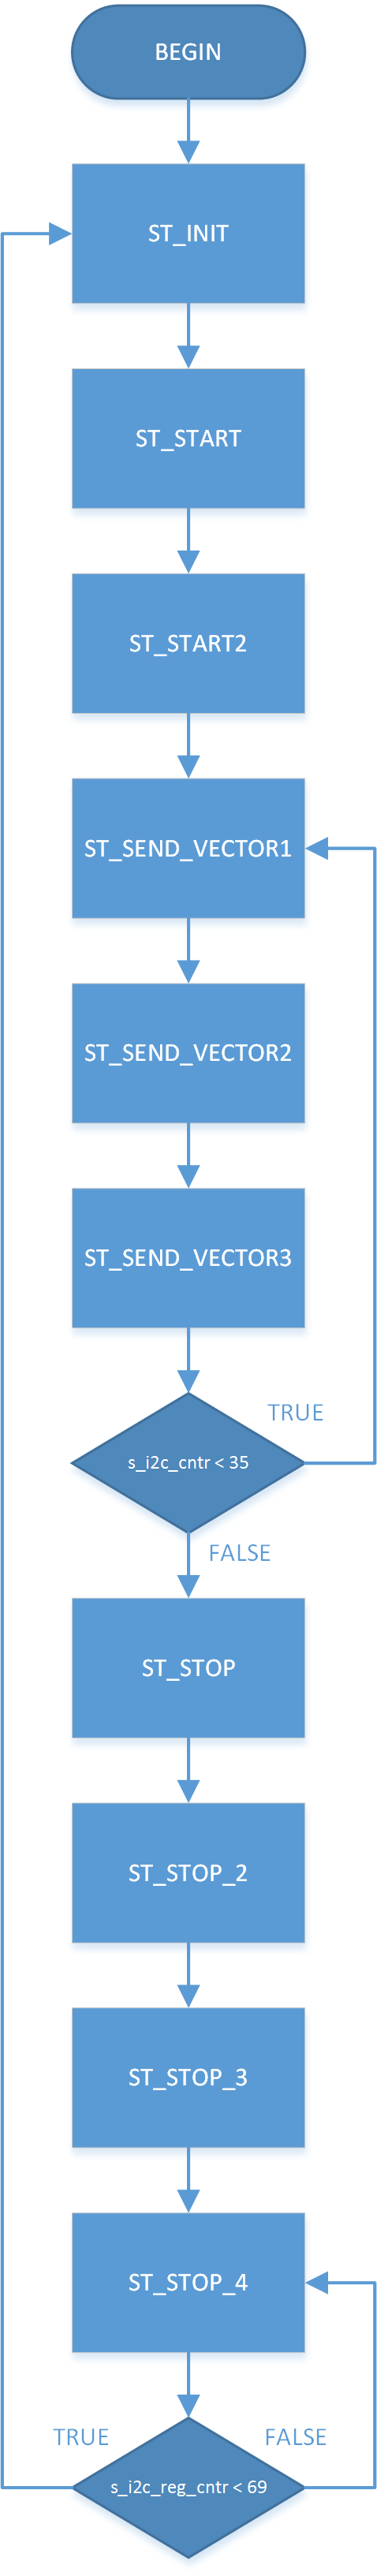
\includegraphics[height=0.85\textheight]{Appendix/FlowCharts/Audio_if}
		\caption{Flowchart van de audio interface}
		\label{fig:FlowChartAudioIF}
	\end{figure}

\newpage
\section{Delay}
\label{sec:appDelay}
	\begin{figure}[H]
		\centering
		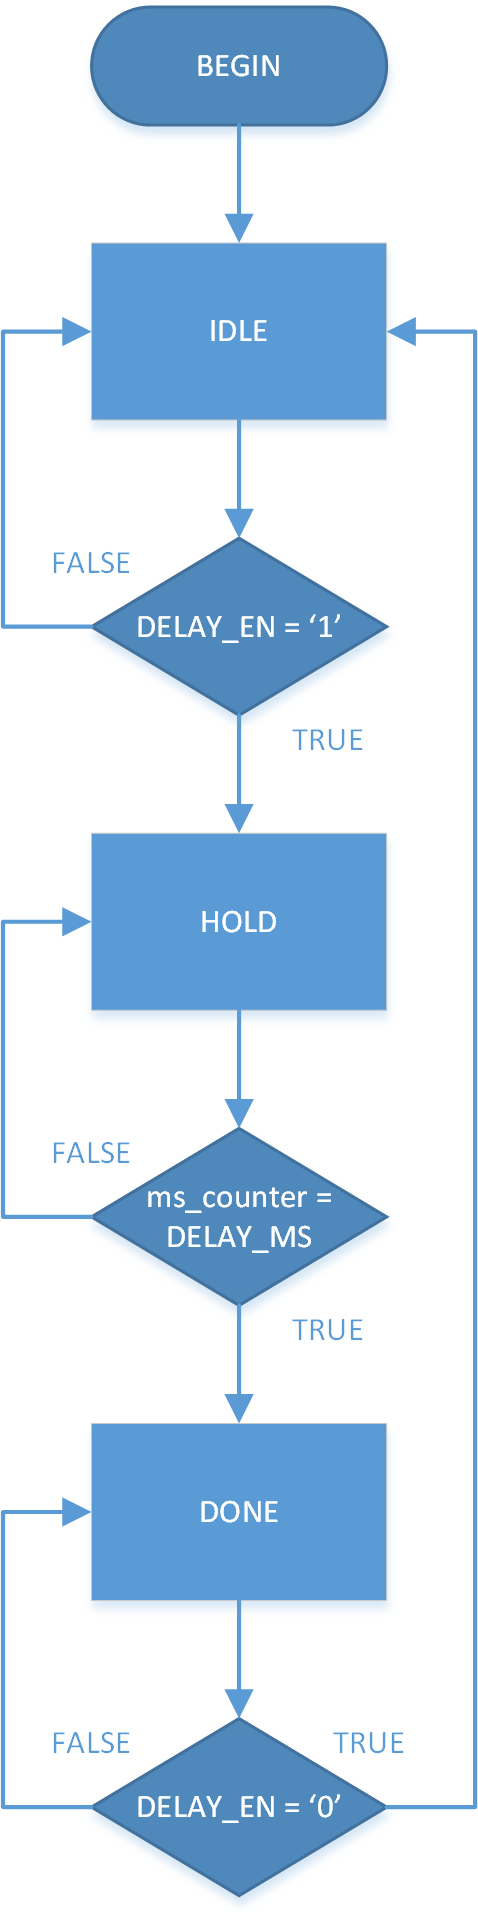
\includegraphics[height=0.85\textheight]{Appendix/FlowCharts/Delay}
		\caption{Flowchart van de audio interface}
		\label{fig:FlowChartDelay}
	\end{figure}

\newpage
\section{Oled top}
\label{sec:appOledTop}
	\begin{figure}[H]
		\centering
		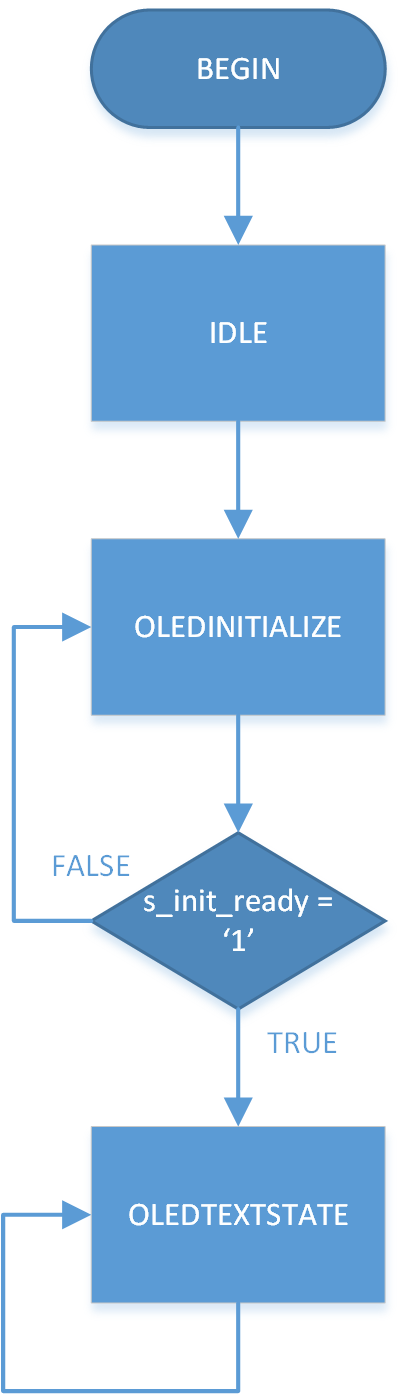
\includegraphics[height=0.85\textheight]{Appendix/FlowCharts/oled_top}
		\caption{Flowchart van oled\textunderscore top}
		\label{fig:FlowChartOledTop}
	\end{figure}

\newpage
\section{Oled initialize}
\label{sec:appOledInit}
	\begin{figure}[H]
		\centering
		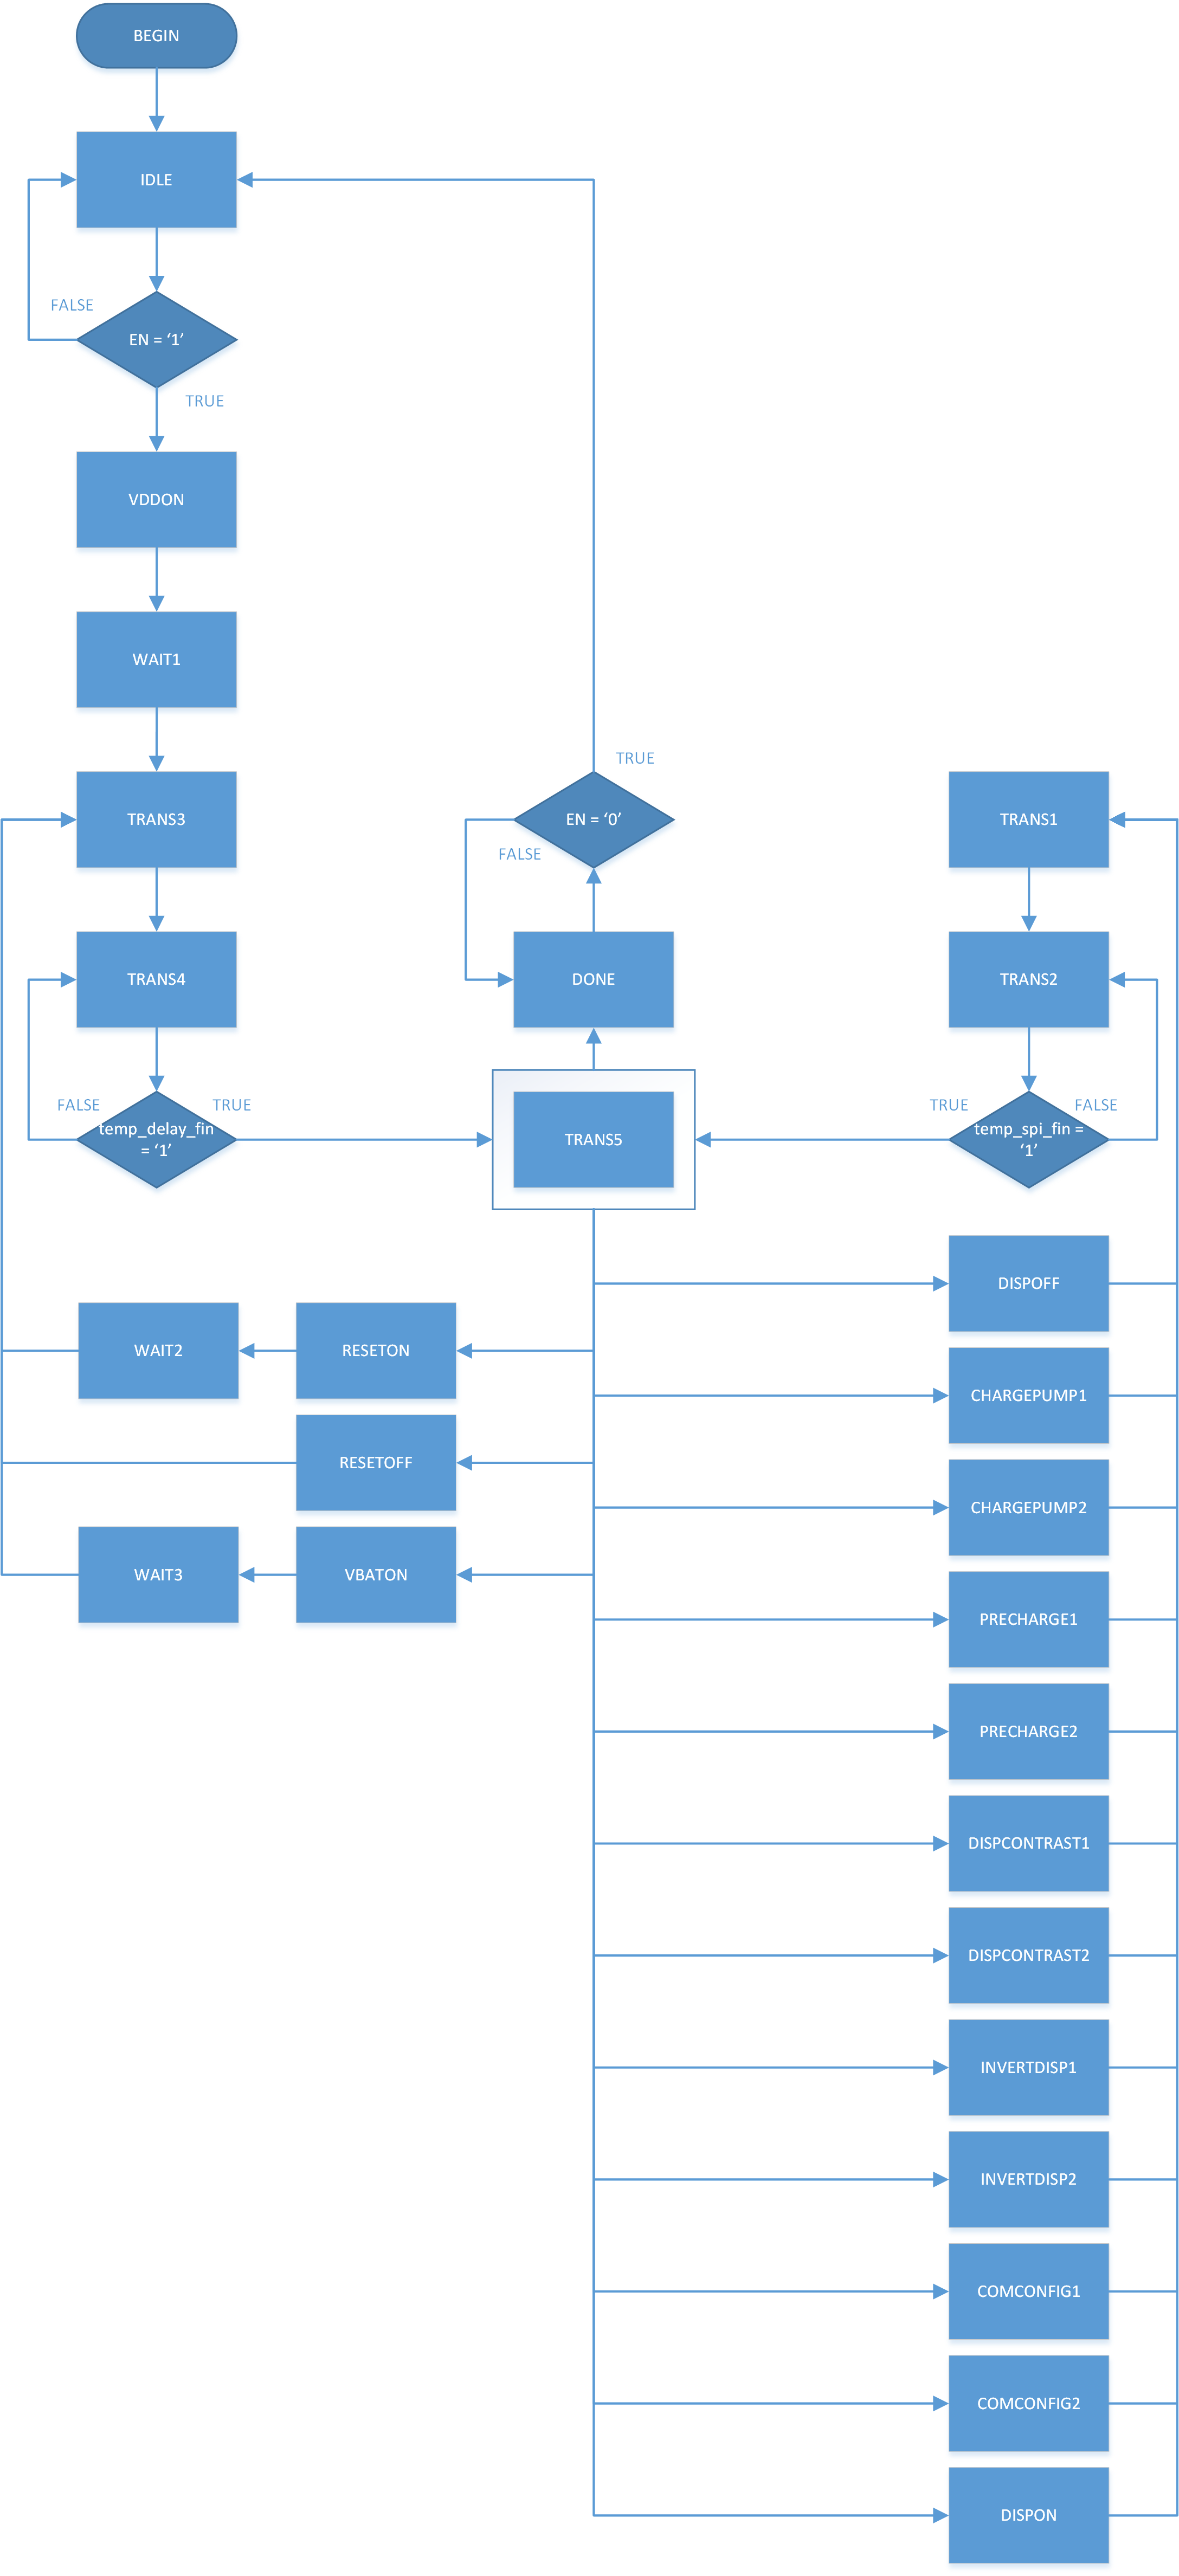
\includegraphics[height=0.85\textheight]{Appendix/FlowCharts/OledInit}
		\caption{Flowchart van OledInit}
		\label{fig:FlowChartOledInit}
	\end{figure}

\newpage
\section{Oled text}
\label{sec:appOledText}
	\begin{figure}[H]
		\centering
		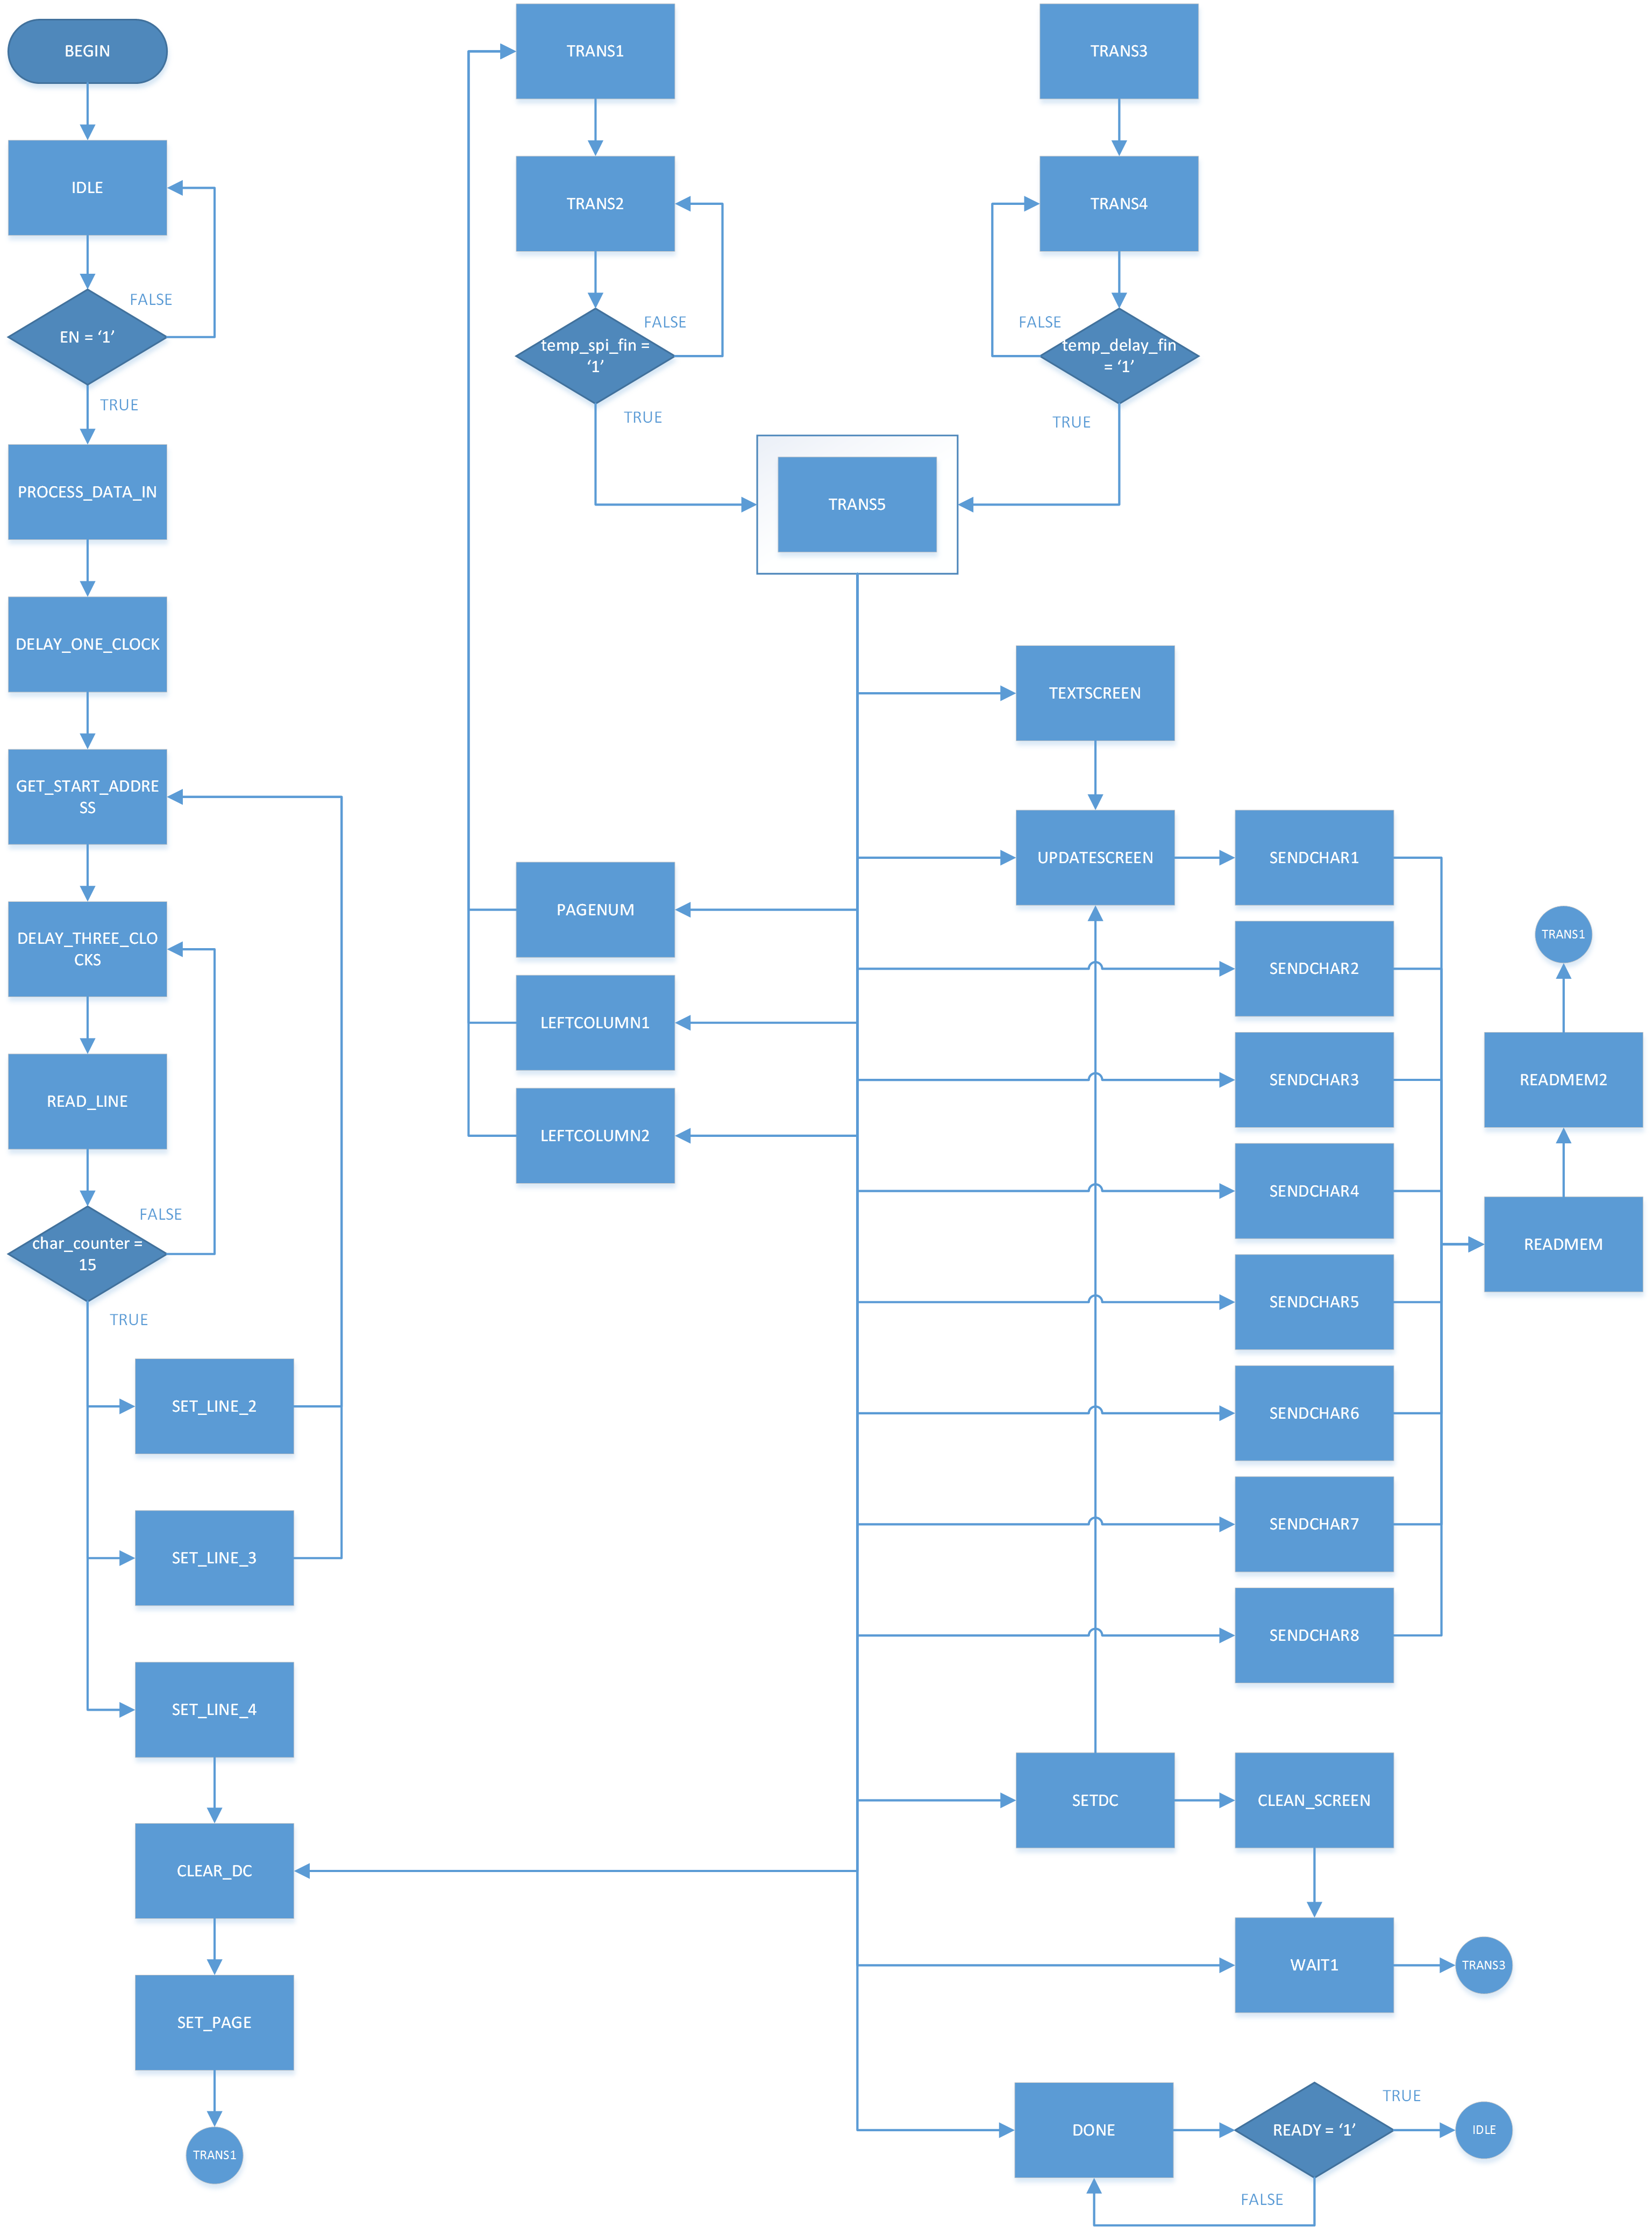
\includegraphics[height=0.85\textheight]{Appendix/FlowCharts/OledText}
		\caption{Flowchart van OledText}
		\label{fig:FlowChartOledText}
	\end{figure}

\newpage
\section{SPI control}
\label{sec:appSpiCtrl}
	\begin{figure}[H]
		\centering
		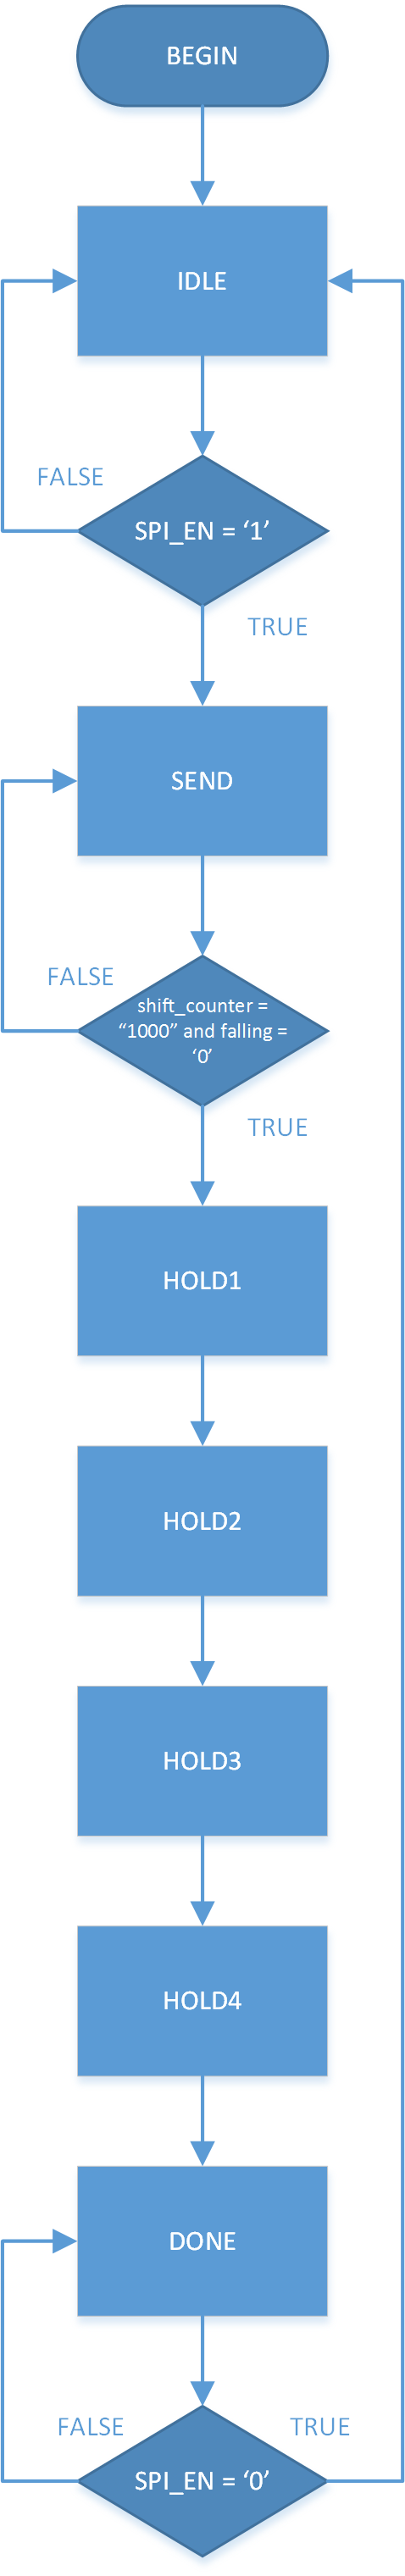
\includegraphics[height=0.85\textheight]{Appendix/FlowCharts/SpiCtrl}
		\caption{Flowchart van SpiCtrl}
		\label{fig:FlowChartSpiCtrl}
	\end{figure}

\chapter{ADAU1761 Settings}
\label{sec:appAdauSettings}
\begin{table}[!htb]
	\footnotesize
    \begin{subtable}{.5\linewidth}
      \centering
        % \caption{}
        \begin{tabular}{l|l}
			Register & Value \\
			\hline
			\hline
			0x4000 & 0x01 \\
			0x4001 & 0x00 \\
			0x4008 & 0x00 \\
			0x4009 & 0x00 \\
			0x400A & 0x01 \\
			0x400B & 0x05 \\
			0x400C & 0x01 \\
			0x400D & 0x05 \\
			0x400E & 0x00 \\
			0x400F & 0x00 \\
			0x4010 & 0x00 \\
			0x4011 & 0x00 \\
			0x4012 & 0x00 \\
			0x4013 & 0x00 \\
			0x4014 & 0x00 \\
			0x4015 & 0x00 \\
			0x4016 & 0x00 \\
			0x4017 & 0x00 \\
			0x4018 & 0x00 \\
			0x4019 & 0x13 \\
			0x401A & 0x00 \\
			0x401B & 0x00 \\
			0x401C & 0x21 \\
			0x401D & 0x00 \\
			0x401E & 0x41 \\
			0x401F & 0x00 \\
			0x4020 & 0x00 \\
			0x4021 & 0x00 \\
			0x4022 & 0x01 \\
			0x4023 & 0xE7 \\
			0x4024 & 0xE7 \\
			0x4025 & 0xE7 \\
			0x4026 & 0xE7 \\
			0x4027 & 0xE7 \\
			0x4028 & 0x00 \\
			\hline
        \end{tabular}
        %\caption{}
    \end{subtable}%
    \begin{subtable}{.5\linewidth}
      \centering
        % \caption{}
        \begin{tabular}{l|l}
			Register & Value \\
			\hline
			\hline
			0x4029 & 0x03 \\
			0x402A & 0x03 \\
			0x402B & 0x00 \\
			0x402C & 0x00 \\
			0x402D & 0xAA \\
			0x402F & 0xAA \\
			0x4030 & 0x00 \\
			0x4031 & 0x08 \\
			0x4036 & 0x03 \\
			0x40C0 & 0x7F \\
			0x40C1 & 0x7F \\
			0x40C2 & 0x7F \\
			0x40C3 & 0x7F \\
			0x40C4 & 0x01 \\
			0x40C6 & 0x00 \\
			0x40C7 & 0x00 \\
			0x40C8 & 0x00 \\
			0x40C9 & 0x00 \\
			0x40D0 & 0x00 \\
			0x40D1 & 0x00 \\
			0x40D2 & 0x00 \\
			0x40D3 & 0x00 \\
			0x40D4 & 0x00 \\
			0x40E9 & 0x10 \\
			0x40EA & 0x00 \\
			0x40EB & 0x7F \\
			0x40F2 & 0x01 \\
			0x40F3 & 0x01 \\
			0x40F4 & 0x00 \\
			0x40F5 & 0x00 \\
			0x40F6 & 0x00 \\
			0x40F7 & 0x00 \\
			0x40F8 & 0x00 \\
			0x40F9 & 0x7F \\
			0x40FA & 0x03 \\
			\hline
        \end{tabular}
        %\caption{}
    \end{subtable}
    \caption{ADAU1761 settings}
\end{table}
\end{document}